% ============================================================
%  Kubernetes Admission Security Operators — IMRAD Presentation
%  Engine: pdflatex + beamer
%  Compile: pdflatex slides.tex (twice for cross-refs)
% ============================================================
\documentclass[aspectratio=169,10pt]{beamer}

% ---------- theme & colours ----------
\usetheme{Madrid}
\usecolortheme{seahorse}
\setbeamertemplate{navigation symbols}{}
\setbeamertemplate{footline}[frame number]

% ---------- packages ----------
\usepackage[T1]{fontenc}
\usepackage[utf8]{inputenc}
\usepackage{lmodern}
\usepackage{listings}
\usepackage{xcolor}
\usepackage{graphicx}
\usepackage{booktabs}
\usepackage{tikz}
\usetikzlibrary{arrows.meta, positioning, shapes.geometric, fit}

% ---------- listing style ----------
\definecolor{codebg}{RGB}{245,247,250}
\definecolor{kwblue}{RGB}{0,112,200}
\definecolor{strgreen}{RGB}{0,128,0}
\definecolor{commentgray}{RGB}{130,130,130}

\lstdefinelanguage{yaml}{
  keywords={apiVersion,kind,metadata,spec,rules,match,validate,
             pattern,name,message,resources,kinds,containers,image,
             labels,limits,memory,cpu,validationFailureAction,
             securityContext,privileged,hostPath,runAsNonRoot,
             runAsUser,allowPrivilegeEscalation,volumes,type,
             hostPID,hostIPC,hostNetwork,deny,conditions,operator,
             value,any,key,preconditions},
  keywordstyle=\color{kwblue}\bfseries,
  sensitive=false,
  comment=[l]{\#},
  commentstyle=\color{commentgray}\itshape,
  stringstyle=\color{strgreen},
  morestring=[b]",
  morestring=[b]',
}

\lstset{
  language=yaml,
  backgroundcolor=\color{codebg},
  basicstyle=\ttfamily\scriptsize,
  breaklines=true,
  frame=single,
  framerule=0.4pt,
  rulecolor=\color{gray!60},
  xleftmargin=4pt,
  xrightmargin=4pt,
  aboveskip=4pt,
  belowskip=2pt,
  showstringspaces=false,
}

\lstdefinestyle{terminal}{
  language={},
  backgroundcolor=\color{black!88},
  basicstyle=\ttfamily\scriptsize\color{green!80!black},
  breaklines=true,
  frame=single,
  framerule=0.4pt,
  rulecolor=\color{black},
  xleftmargin=4pt,
  xrightmargin=4pt,
  aboveskip=4pt,
  belowskip=2pt,
  showstringspaces=false,
}

% ---------- metadata ----------
\title{Kubernetes Admission Security Operators}
\subtitle{Policy Enforcement via Admission Controllers \& Kyverno}
\author{k8s-kyverno-demo}
\date{March 2026}
\institute{Kubernetes Security}

% ============================================================
\begin{document}
% ============================================================

% ---- Slide 1: Title ----------------------------------------
\begin{frame}
  \titlepage
\end{frame}

% ---- Slide 2: Outline --------------------------------------
\begin{frame}{Outline}
  \tableofcontents[hideallsubsections]
\end{frame}

% ============================================================
\section{Introduction}
% ============================================================

% ---- Slide 3: Problem Statement ----------------------------
\begin{frame}{Introduction — The Shared-Cluster Problem}
  \begin{columns}[T]
    \column{0.55\textwidth}
      \textbf{Why cluster-wide policy enforcement?}
      \begin{itemize}
        \item Many teams share a single Kubernetes cluster
        \item \texttt{kubectl apply} gives users broad power
        \item Common misconfigurations in practice:
          \begin{itemize}
            \item \texttt{nginx:latest} — unpinned, drifts silently
            \item No CPU/memory limits → noisy-neighbour DoS
            \item Privileged containers → full node escape
            \item Missing labels → invisible to monitoring
          \end{itemize}
        \item \textbf{Goal:} automatically \emph{reject} non-compliant
              workloads before they reach \texttt{etcd}
      \end{itemize}
    \column{0.42\textwidth}
      \begin{alertblock}{Container Escape Risk}
        A container running as \texttt{root} with \texttt{privileged: true}
        and a \texttt{hostPath} volume can:
        \begin{itemize}
          \item Read/write host filesystem
          \item Access node credentials
          \item Pivot to the control plane
        \end{itemize}
        This is a \textbf{critical} threat in multi-tenant clusters.
      \end{alertblock}
  \end{columns}
\end{frame}

% ============================================================
\section{Background}
% ============================================================

% ---- Slide 4: Admission Controller Architecture ------------
\begin{frame}{Background — Kubernetes Admission Controller Pipeline}
  \begin{center}
  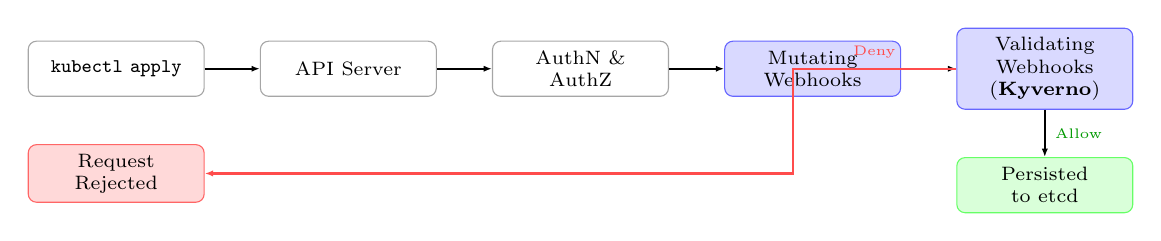
\begin{tikzpicture}[
    node distance=0.55cm and 0.7cm,
    box/.style={rectangle, rounded corners=3pt, draw=gray!70,
                fill=white, text width=2.0cm, align=center,
                font=\scriptsize, minimum height=0.7cm},
    webhook/.style={box, fill=blue!15, draw=blue!60},
    danger/.style={box, fill=red!15, draw=red!60},
    ok/.style={box, fill=green!15, draw=green!60},
    arr/.style={-{Latex[length=3pt]}, thick},
  ]
    \node[box]  (user)   {\texttt{kubectl apply}};
    \node[box, right=of user]   (api)    {API Server};
    \node[box, right=of api]    (authn)  {AuthN \& AuthZ};
    \node[webhook, right=of authn] (mut) {Mutating\\ Webhooks};
    \node[webhook, right=of mut]   (val) {Validating\\ Webhooks\\ (\textbf{Kyverno})};
    \node[ok,   below=0.6cm of val]  (etcd)   {Persisted\\ to etcd};
    \node[danger, below=0.6cm of user] (reject) {Request\\ Rejected};

    \draw[arr] (user)  -- (api);
    \draw[arr] (api)   -- (authn);
    \draw[arr] (authn) -- (mut);
    \draw[arr] (mut)   -- (val);
    \draw[arr] (val)   -- node[right, font=\tiny\color{green!60!black}]{Allow} (etcd);
    \draw[arr, red!70] (val) -- node[above, font=\tiny\color{red}]{Deny} +(-3.2,0) |- (reject);
  \end{tikzpicture}
  \end{center}

  \begin{columns}[T]
    \column{0.48\textwidth}
      \textbf{ValidatingAdmissionWebhook}
      \begin{itemize}
        \item Called \emph{before} persisting any resource
        \item Returns \texttt{allowed: true/false} + reason
        \item Kyverno registers itself as one automatically
      \end{itemize}
    \column{0.48\textwidth}
      \textbf{Why Kyverno?}
      \begin{itemize}
        \item Policies are plain YAML — no Rego/Go required
        \item Runs fully in-cluster as a Deployment
        \item Covers: validate, mutate, generate, verify-image
      \end{itemize}
  \end{columns}
\end{frame}

% ============================================================
\section{Methods}
% ============================================================

% ---- Slide 5: Setup & Installation -------------------------
\begin{frame}[fragile]{Methods — Environment Setup}
  \begin{columns}[T]
    \column{0.50\textwidth}
      \textbf{Toolchain}
      \begin{itemize}
        \item Minikube (local single-node cluster)
        \item Helm (Kyverno package manager)
        \item kubectl (resource management)
        \item Makefile for reproducibility
      \end{itemize}
      \vspace{4pt}
      \textbf{One-command setup:}
\begin{lstlisting}[style=terminal]
$ make start
# Starts Minikube, installs Kyverno
# via Helm, applies all policies
\end{lstlisting}
    \column{0.48\textwidth}
\begin{lstlisting}
# Makefile excerpt
start:
  minikube start
  helm repo add kyverno \
    https://kyverno.github.io/kyverno/
  helm repo update
  helm upgrade --install kyverno \
    kyverno/kyverno \
    -n kyverno --create-namespace
  # Wait up to 20 retries x 5 s
  kubectl wait --for=condition=available\
    deployment --all -n kyverno \
    --timeout=120s
  kubectl apply -f policies/
\end{lstlisting}
  \end{columns}
\end{frame}

% ---- Slide 6: Policy 1 — Disallow latest tag ---------------
\begin{frame}[fragile]{Methods — Policy 1: Disallow \texttt{latest} Image Tag}
  \begin{columns}[T]
    \column{0.50\textwidth}
\begin{lstlisting}[title=policies/policy.yaml]
apiVersion: kyverno.io/v1
kind: ClusterPolicy
metadata:
  name: disallow-latest-tag
spec:
  validationFailureAction: Enforce
  rules:
    - name: check-image-tag
      match:
        resources:
          kinds:
            - Pod
      validate:
        message: "latest tag is not allowed"
        pattern:
          spec:
            containers:
              - image: "!*:latest"
\end{lstlisting}
    \column{0.47\textwidth}
      \textbf{Rationale}
      \begin{itemize}
        \item \texttt{latest} is mutable — image content can change
              between pulls silently
        \item Supply-chain attack vector: a compromised registry
              can replace \texttt{latest} with malicious content
        \item Breaks reproducibility: two identical manifests may
              run different binaries
      \end{itemize}
      \vspace{4pt}
      \textbf{Pattern logic:} \texttt{"!\,*:latest"} rejects any image
      whose tag is exactly \texttt{latest}; explicit semver tags
      (\texttt{nginx:1.25.3}) are accepted.
  \end{columns}
\end{frame}

% ---- Slide 7: Policy 2 & 3 ---------------------------------
\begin{frame}[fragile]{Methods — Policies 2 \& 3: Labels and Resource Limits}
  \begin{columns}[T]
    \column{0.50\textwidth}
\begin{lstlisting}[title=policies/policy-requires-labels.yaml]
apiVersion: kyverno.io/v1
kind: ClusterPolicy
metadata:
  name: require-app-label
spec:
  validationFailureAction: Enforce
  rules:
    - name: check-label
      match:
        resources:
          kinds: [Pod]
      validate:
        message: "app label is required"
        pattern:
          metadata:
            labels:
              app: "?*"
\end{lstlisting}
    \column{0.47\textwidth}
\begin{lstlisting}[title=policies/policy-resources.yaml]
apiVersion: kyverno.io/v1
kind: ClusterPolicy
metadata:
  name: require-resources
spec:
  validationFailureAction: Enforce
  rules:
    - name: check-resources
      match:
        resources:
          kinds: [Pod]
      validate:
        message: >
          CPU and memory limits required
        pattern:
          spec:
            containers:
              - resources:
                  limits:
                    memory: "?*"
                    cpu: "?*"
\end{lstlisting}
  \end{columns}
\end{frame}

% ---- Slide 8: Policy 4 — Container Escape Prevention ------
\begin{frame}[fragile]{Methods — Policy 4: Prevent Container Escapes}
  \begin{columns}[T]
    \column{0.50\textwidth}
\begin{lstlisting}[title=policies/policy-security-context.yaml]
apiVersion: kyverno.io/v1
kind: ClusterPolicy
metadata:
  name: disallow-privileged-containers
spec:
  validationFailureAction: Enforce
  rules:
    - name: no-privileged
      match:
        resources:
          kinds: [Pod]
      validate:
        message: >
          Privileged containers not allowed.
          Use a non-root, non-privileged
          security context.
        pattern:
          spec:
            containers:
              - securityContext:
                  privileged: "false | !exists"
                  allowPrivilegeEscalation:
                    "false | !exists"
                  runAsNonRoot: true
            volumes:
              - =(type): "!hostPath"
\end{lstlisting}
    \column{0.47\textwidth}
      \textbf{Threat model}
      \begin{itemize}
        \item \texttt{privileged: true} gives container
              \emph{full} host capabilities (CAP\_SYS\_ADMIN)
        \item \texttt{hostPath} mounts expose the node FS
              including kubelets, SSH keys, tokens
        \item \texttt{runAsRoot} + writable FS → escape via
              \texttt{nsenter}, \texttt{chroot}, \texttt{/proc}
        \item \texttt{allowPrivilegeEscalation} enables
              \texttt{setuid} binaries inside container
      \end{itemize}
      \vspace{4pt}
      \begin{block}{Defence-in-depth}
        This policy complements Pod Security Admission
        (PSA) and Linux seccomp/AppArmor profiles,
        stopping misconfigured workloads \emph{at entry}.
      \end{block}
  \end{columns}
\end{frame}

% ---- Slide 9: Policy 5 — Sensitive Host Mounts -------------
\begin{frame}[fragile]{Methods — Policy 5: Block Sensitive Host Mounts}
  \begin{columns}[T]
    \column{0.50\textwidth}
\begin{lstlisting}[title=policies/policy-sensitive-mounts.yaml]
apiVersion: kyverno.io/v1
kind: ClusterPolicy
metadata:
  name: disallow-sensitive-mounts
spec:
  validationFailureAction: Enforce
  rules:
    - name: check-sensitive-paths
      match:
        resources:
          kinds: [Pod]
      validate:
        message: >
          Sensitive host path mount detected.
          Mounting docker socket, host creds
          or /proc is forbidden.
        deny:
          conditions:
            any:
            - key: "{{ request.object.spec\
  .volumes[].hostPath.path }}"
              operator: AnyIn
              value:
              - /var/run/docker.sock
              - /var/run/crio/crio.sock
              - /etc/kubernetes
              - /etc/shadow
              - /root
              - /proc
              - /sys/fs/cgroup
\end{lstlisting}
    \column{0.47\textwidth}
      \textbf{Attack scenario}
      \begin{itemize}
        \item Mount \texttt{/var/run/docker.sock} $\Rightarrow$
              full Docker daemon access from inside container;
              attacker runs \texttt{docker run -{}-privileged}
              to get root on the node
        \item Mount \texttt{/etc/kubernetes} $\Rightarrow$
              reads admin \texttt{kubeconfig} / service-account tokens
        \item Mount \texttt{/proc} $\Rightarrow$
              read memory of any host process via
              \texttt{/proc/<pid>/mem}
      \end{itemize}
      \vspace{4pt}
\begin{lstlisting}[style=terminal,title=Rejection output]
$ kubectl apply -f spy-pod.yaml

Error from server: admission webhook
"validate.kyverno.svc-fail" denied
the request:

resource Pod/default/spy-pod was
blocked due to the following policies:

disallow-sensitive-mounts:
  check-sensitive-paths: Sensitive
  host path mount detected. Mounting
  docker socket, host creds or /proc
  is forbidden.
\end{lstlisting}
  \end{columns}
\end{frame}

% ---- Slide 10: Policy 6 — Host PID / Shared Procfs ---------
\begin{frame}[fragile]{Methods — Policy 6: Prevent Host PID / Shared Procfs}
  \begin{columns}[T]
    \column{0.50\textwidth}
\begin{lstlisting}[title=policies/policy-host-namespaces.yaml]
apiVersion: kyverno.io/v1
kind: ClusterPolicy
metadata:
  name: disallow-host-namespaces
spec:
  validationFailureAction: Enforce
  rules:
    - name: check-host-pid-ipc
      match:
        resources:
          kinds: [Pod]
      validate:
        message: >
          hostPID/hostIPC/hostNetwork share
          the host's process table, IPC, and
          network -- all forbidden in this
          cluster.
        pattern:
          spec:
            =(hostPID): "false"
            =(hostIPC): "false"
            =(hostNetwork): "false"
\end{lstlisting}
    \column{0.47\textwidth}
      \textbf{Attack scenario}
      \begin{itemize}
        \item \texttt{hostPID: true} $\Rightarrow$ container sees
              \emph{all} host PIDs; attacker reads
              \texttt{/proc/<pid>/environ} for secrets/tokens
              and can \texttt{ptrace} or \texttt{kill}
              arbitrary processes
        \item \texttt{hostNetwork: true} $\Rightarrow$ sniff raw
              node traffic; reach the metadata API
              (\texttt{169.254.169.254}) for cloud credentials
        \item \texttt{hostIPC: true} $\Rightarrow$ attach to shared
              memory segments of other workloads
      \end{itemize}
      \vspace{4pt}
\begin{lstlisting}[style=terminal,title=Rejection output]
$ kubectl apply -f proc-spy-pod.yaml

Error from server: admission webhook
"validate.kyverno.svc-fail" denied
the request:

resource Pod/default/proc-spy was
blocked due to the following policies:

disallow-host-namespaces:
  check-host-pid-ipc: hostPID/hostIPC/
  hostNetwork share the host's process
  table, IPC, and network -- all
  forbidden in this cluster.
\end{lstlisting}
  \end{columns}
\end{frame}

% ============================================================
\section{Results}
% ============================================================

% ---- Slide 11: Test Manifest & Rejection Output -------------
\begin{frame}[fragile]{Results — Non-Compliant Workload \& Rejection}
  \begin{columns}[T]
    \column{0.46\textwidth}
\begin{lstlisting}[title=test/deployment.yaml (non-compliant)]
apiVersion: apps/v1
kind: Deployment
metadata:
  name: nginx-test
spec:
  replicas: 1
  selector:
    matchLabels:
      app: nginx
  template:
    metadata:
      labels:
        app: nginx
    spec:
      containers:
      - name: nginx
        image: nginx:latest  # VIOLATION
        # No resource limits  # VIOLATION
        # No securityContext  # VIOLATION
\end{lstlisting}
    \column{0.52\textwidth}
      \textbf{Admission controller output:}
\begin{lstlisting}[style=terminal]
$ kubectl apply -f test/deployment.yaml

Error from server:
admission webhook
"validate.kyverno.svc-fail" denied
the request:

resource Deployment/default/nginx-test
was blocked due to the following
policies:

disallow-latest-tag:
  check-image-tag: latest tag is
  not allowed

require-resources:
  check-resources: CPU and memory
  limits are required
\end{lstlisting}
      \vspace{2pt}
      \small{The request never reaches \texttt{etcd} — zero runtime exposure.}
  \end{columns}
\end{frame}

% ---- Slide 10: Policy Coverage Matrix ----------------------
\begin{frame}{Results — Policy Coverage Matrix}
  \begin{center}
  \renewcommand{\arraystretch}{1.35}
  \begin{tabular}{lllc}
    \toprule
    \textbf{Policy} & \textbf{Threat Addressed} & \textbf{Action} & \textbf{Scope} \\
    \midrule
    \texttt{disallow-latest-tag}      & Supply-chain / image drift        & Enforce & ClusterPolicy \\
    \texttt{require-app-label}        & Observability gap                 & Enforce & ClusterPolicy \\
    \texttt{require-resources}        & Resource starvation / DoS         & Enforce & ClusterPolicy \\
    \texttt{disallow-privileged}      & Container escape (root/caps)      & Enforce & ClusterPolicy \\
    \texttt{disallow-sensitive-mounts}& Docker socket / host cred theft   & Enforce & ClusterPolicy \\
    \texttt{disallow-host-namespaces} & Procfs spy / network sniff        & Enforce & ClusterPolicy \\
    \bottomrule
  \end{tabular}
  \end{center}

  \vspace{6pt}
  \begin{columns}[T]
    \column{0.48\textwidth}
      \textbf{Compliant workload (accepted):}
      \begin{itemize}
        \item Image: \texttt{nginx:1.25.3}
        \item Labels: \texttt{app: nginx}
        \item Limits: \texttt{cpu: 200m, memory: 128Mi}
        \item \texttt{runAsNonRoot: true, privileged: false}
      \end{itemize}
    \column{0.48\textwidth}
      \textbf{Blocked scenarios (rejected):}
      \begin{itemize}
        \item Any \texttt{:latest} tagged image
        \item Pod without \texttt{app} label
        \item Container without CPU/memory limits
        \item Privileged or root container
        \item \texttt{hostPath} volume mounts
        \item Sensitive path mounts (\texttt{docker.sock}, \texttt{/etc/kubernetes}, \texttt{/proc})
        \item \texttt{hostPID}/\texttt{hostIPC}/\texttt{hostNetwork} sharing
      \end{itemize}
  \end{columns}
\end{frame}

% ============================================================
\section{Discussion}
% ============================================================

% ---- Slide 11: Discussion ----------------------------------
\begin{frame}{Discussion — Findings, Limitations \& Future Work}
  \begin{columns}[T]
    \column{0.48\textwidth}
      \textbf{Key Findings}
      \begin{itemize}
        \item Kyverno integrates in minutes via Helm with \emph{zero} custom code
        \item \texttt{validationFailureAction: Enforce} blocks at the API layer —
              no workload ever starts
        \item Policies are auditable plain YAML, suitable for GitOps (ArgoCD/Flux)
        \item Container escape prevention closes critical multi-tenant attack paths
      \end{itemize}
      \vspace{6pt}
      \textbf{Limitations}
      \begin{itemize}
        \item Policies currently target \texttt{Pod} kind only;
              \texttt{Deployment}/\texttt{DaemonSet} require additional rules
        \item No image vulnerability scanning (CVE-level)
        \item Kyverno is a SPOF unless deployed in HA mode ($\ge$3 replicas)
        \item \texttt{Audit} mode needed before \texttt{Enforce} in brownfield clusters
      \end{itemize}
    \column{0.48\textwidth}
      \textbf{Future Work}
      \begin{itemize}
        \item \textbf{Image verification} — cosign signatures + Kyverno
              \texttt{verifyImages} rules
        \item \textbf{Vulnerability scanning} — Trivy Operator +
              Kyverno \texttt{generate} to block known-CVE images
        \item \textbf{Mutation rules} — auto-inject resource defaults
              and non-root security context
        \item \textbf{Network isolation} — \texttt{NetworkPolicy} generation
              per namespace via Kyverno
        \item \textbf{Runtime enforcement} — Falco / Tetragon for
              post-admission behavioural anomaly detection
        \item \textbf{Policy-as-Code CI} — \texttt{kyverno test} in
              GitHub Actions / GitLab CI pipelines
      \end{itemize}
  \end{columns}
\end{frame}

% ---- Slide 12: Conclusion ----------------------------------
\begin{frame}{Conclusion}
  \begin{block}{Summary}
    Kubernetes admission controllers — implemented here via Kyverno — provide a
    \textbf{preventive, policy-as-code layer} that stops non-compliant and
    potentially malicious workloads \emph{before} they are scheduled, with no
    runtime overhead.
  \end{block}

  \vspace{8pt}

  \begin{columns}[T]
    \column{0.30\textwidth}
      \textbf{Implemented}
      \begin{itemize}
        \item Image tag pinning
        \item Mandatory labels
        \item Resource limits
        \item Privilege/escape prevention
      \end{itemize}
    \column{0.30\textwidth}
      \textbf{Mechanisms}
      \begin{itemize}
        \item ValidatingAdmissionWebhook
        \item Kyverno ClusterPolicy
        \item Helm + Makefile automation
        \item One-command reproducibility
      \end{itemize}
    \column{0.36\textwidth}
      \textbf{Takeaway}
      \begin{itemize}
        \item Shift security \textbf{left}: enforce at admission,
              not at runtime
        \item Policies are code — version, review, test them
        \item Layer defences: PSA + Kyverno + runtime tools
        \item Start in \texttt{Audit} mode, graduate to \texttt{Enforce}
      \end{itemize}
  \end{columns}

  \vspace{10pt}
  \begin{center}
    \small
    \textbf{Repository:} \texttt{k8s-kyverno-demo} \quad
    \textbf{Stack:} Minikube · Kyverno · Helm · kubectl \\[4pt]
    \textit{"Security is a process, not a product — but a good admission controller is a fine start."}
  \end{center}
\end{frame}

% ============================================================
\end{document}
